\renewcommand*{\mypath}{trovaintruso1}%
\graphicspath{ {\mypath/images/} }

\doctitle{Paolo Ferraris}{paolo2.ferraris@mail.polimi.it}
\localtoc

\section{Descrizione delle classi}

\noindent Per prima cosa vengono descritte le classi principali, partendo dal modello che definisce il gioco, in seguito vengono descritte le classi Helper che permettono la gestione della logica, e infine le Activity utilizzate.

\subsection{Classi del modello dati}

\noindent Di seguito sono descritte le classi che gestiscono il modello del gioco, rappresentate nel class diagram della Figura \ref{fig:class_diagram}:

\begin{figure}
	\centering
	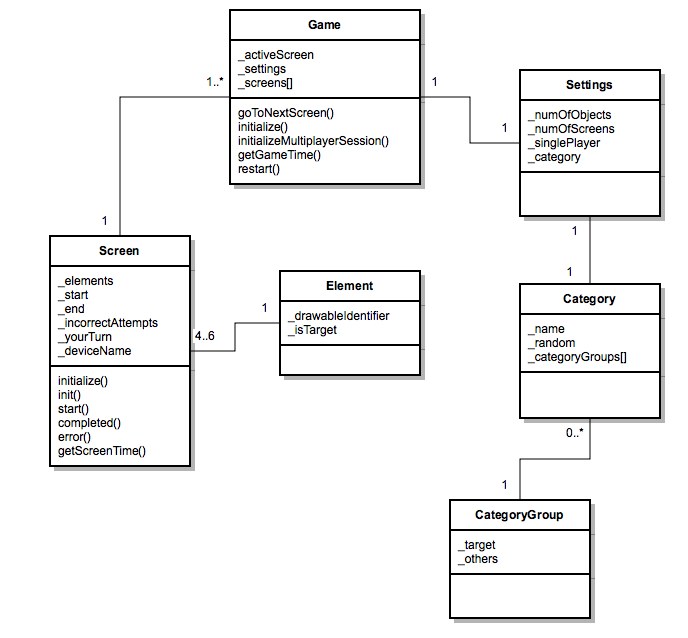
\includegraphics[width=13.5cm]{trova_l_intruso_class_diagram}
	\caption{Class Diagram}
	\label{fig:class_diagram}
\end{figure}
\begin{description}
\item \textbf{Game} \`{e} la classe che gestisce la partita, i principali metodi sono:
\begin{itemize}
\item initialize(): metodo che inizializza la sessione di gioco, creando i livelli e assegnandone gli oggetti da visualizzare.
\item initializeMultiplayerSession(boolean guest): metodo che stabilisce i turni di gioco nelle partite multiplayer, la variabile guest indica se il dispositivo \`{e} quello che \`{e} stato invitato a giocare.
\item goToNextScreen(): metodo che attiva la schermata successiva e restituisce true. Nel caso ci si trovi nell'ultimo livello restituisce false.
\item fillScreens(): riempie le schermate con le immagini in base alla categoria e al numero di oggetti da visualizzare.
\item CreateGameDescription(Context context): crea la descrizione della partita da mandare via mail.
\item restart(): riavvia il gioco con le stesse impostazioni.
\end{itemize}
\item \textbf{Settings} Classe che gestisce le impostazioni di gioco, possiede le seguenti propriet\`{a}:
\begin{itemize}
\item \_singlePlayer(Boolean): indica la modalit\`{a} di gioco.
\item \_numOfObjects(int): indica il numero di immagini visualizzate per livello.
\item \_numOfScreens(int): indica il numero di livelli impostati.
\item \_category(Category): indica la categoria di immagini selezionata.
\end{itemize}

\item \textbf{Screen}
Classe che rappresenta il livello di gioco, possiede come propeirt\`{a} il tempo di inzio livello, il tempo di fine, una variabile booleana che indica se \`{e} il turno del giocatore corrente, il numero di errori e un array contenente le immagini da visualizzare. I principali metodi sono:
\begin{itemize}
\item initialize(): inizializza il livello, inserendo le immagini.
\item init(): azzera le variabili del livello, ossia numero di errori, tempo di gioco.
\item start(): avvia il gioco su questo livello, settando la variabile \_start\_time.
\item error(): incrementa il conteggio degli errori di uno.
\item completed(): metodo evocato quando il livello \`{e} completato, setta la variabile \_end\_time.
\item getScreenTime(): restituisce il tempo di gioco.
\end{itemize}
\item \textbf{Element}
\noindent Classe che rappresenta un immagine, possiede due attributi, il nome dell'immagine presente nella cartella \emph{drawable} e un valore booleano che indica se \`{e} l'elemento target.
\item \textbf{Category}
Classe che rappresenta una categoria di immagini, possiede come propriet\`{a} il nome della categoria, un campo booleano che indica se si tratta di una categoria "Casuale" e una lista di oggetti CategoryGroups relativi alla categoria. Il costruttore accetta un JSONObject contenente la definizione della categoria e da esso inizializza l'oggetto.
\item \textbf{CategoryGroup}
Classe che rappresenta una gruppo di immagini che deve essere rappresentato in una schermata. Definisce l'elemento target e i restanti elementi.
\end{description}

\subsection{Classi Helper}

\begin{description}
\item \textbf{CategoryHelper} Gestisce il caricamento delle categorie di immagini dal file .json dove sono definite.
\item \textbf{GameHelper} Gestisce le meccaniche di gioco e la comunicazione tra i dispositivi in multiplayer. I principali metodi di questa classe sono:
\begin{itemize}
\item onMainActivityCreate(): metodo utilizzato all'avvio dell'activity principale, avvia il riconoscimento dei dispositivi sul network (per le partite in multiplayer) e carica le impostazioni di gioco precedentemente salvate.
\item onMainActivityDestroy(): chiamato quando l'activity principale viene distrutta, viene terminato il servizio di discovery sul network e viene chiusa la connessione (se attiva).
\item registerCurrentActivity(Activity activity): metodo chiamato nell'onCreate di ogni activity, registra l'activity mostrata a schermo per gestire al meglio le comunicazioni tra i dispositivi in multiplayer e la visualizzazione di avvisi o dei feedback di gioco.
\item startGame(): Questo metodo inizializza il gioco, viene chiamato il metodo Game.initialize() e in seguito se il gioco \`{e} in SinglePlayer viene caricata l'activity Screen nella quale viene mostrato il primo livello, altrimenti si passa all'activity MultiPlayerDiscoveryActivity per invitare un giocatore.
\item quitGame(): questo metodo serve per terminare una partita, e nel caso di partite multiplayer viene chiusa anche la connessione.
\item nextScreen(): metodo che serve per passare al livello successivo, in caso di partite multiplayer viene inviato l'analogo messaggio all'altro dispositivo.
\end{itemize}
\item \textbf{MultiPlayerServiceHelper} Gestisce il riconoscimento dei dispositivi che eseguono il gioco sulla rete per permettere l'avvio di partite multiplayer.
\item \textbf{ConnectionHelper} Il multiplayer \`{e} implementato usando i socket Java, questa classe gestisce la connessione, l'invio di messaggi sul network e inizializza gli oggetti ServerHelper e ClientHelper.
\item \textbf{ServerHelper} Gestisce il lato server della connessione, avviando un SocketServer thread che si occupa dell'assegnamento di una connessione al socket client appena arriva una richiesta al server.
\item \textbf{ClientHelper} Questa classe istanzia due thread, un thread che si occupa della ricezione dei messaggi in arrivo al socket utilizzato per la connessione, e uno che si occupa di inviare i messaggi al dispositivo col quale si sta giocando.
\end{description}

\subsection{Gestione della comunicazione in partite multiplayer}
\noindent Per la gestione delle comunicazioni tra dispositivi nelle partite multiplayer \`{e} stata creata una classe GameMessage, la quale definisce una propriet\`{a} di tipo Serializable, che rappresenta il contenuto del messaggio, e una propriet\`{a} chiamata "Type", un enum che indica il tipo di messaggio, che pu\`{o} assumere i seguenti valori:
\begin{itemize}
\item \emph{ConnectionRequest}: i messaggi di questo tipo non hanno contenuto e servono ad inoltrare a un dispositivo una richiesta di connessione per avviare una partita;
\item \emph{ConncectionAccepted}: questo messaggio viene inviato dal client al server quando il giocatore accetta di giocare;
\item \emph{ConncectionClosed}: questo messaggio viene inviato prima di chiudere la connessione;
\item \emph{SendGame}: con questo messaggio viene inviata la struttura del gioco al dispositivo invitato a giocare;
\item \emph{SendGameAck}: questo messaggio conferma la ricezione del messaggio precedente da parte del client;
\item \emph{StartGame}: questo messaggio viene inviato al dispositivo client per comunicargli di avviare il gioco, alla sua ricezione il client avvia il gioco e manda il messaggio di ack al server;
\item \emph{StartGameAck}: questo messaggio conferma la ricezione del messaggio precedente, alla sua ricezione il dispositivo server a sua volta avvia il gioco;
\item \emph{ElementPressed}: con questo messaggio viene inviato l'indice dell'elemento premuto all'altro dispositivo in modo da visualizzare il feedback;
\item \emph{NextScreen}: con questo messaggio si comunica al dispositivo avversario che il giocatore ha premuto il pulsante per cambiare schermata.
\end{itemize}

\subsection{Activity}

\noindent Di seguito vengono descritte le principali Activity presenti nell'app:

\begin{description}
\item \textbf{MainActivity}: \`{e} l'activity che si presenta all'avvio del gioco, inizializza la propriet\`{a} globale GameHelper e permette di avviare il gioco.
\item \textbf{ScreenActivity}: l'activity che gestisce il livello di gioco, all'avvio vengono caricate le immagini e mostrate a schermo, in seguito si attende l'input dell'utente e si visualizzano a schermo i feedback.
\item \textbf{ResultsActivity}: l'activity che viene mostrata alla fine del gioco, mostra i risultati dei livelli e permette di riavviare il gioco oppure tornare alla MainActivity.
\item \textbf{MultiPlayerDiscoveryActivity}: in questa activity vengono mostrati gli altri giocatori e si pu\`{o} iniziare una partita multiplayer.
\item \textbf{SettingsActivity} e \textbf{ConfigDeviceActivity} permettono la configurazione delle impostazioni della partita e del dispositivo.
\end{description}

\section{Modello della sessione di gioco}

\noindent
Nella Figura \ref{fig:activity_diagram} \`{e} riportato l'activity diagram che schematizza lo svolgimento del gioco.

\begin{figure}
	\centering
    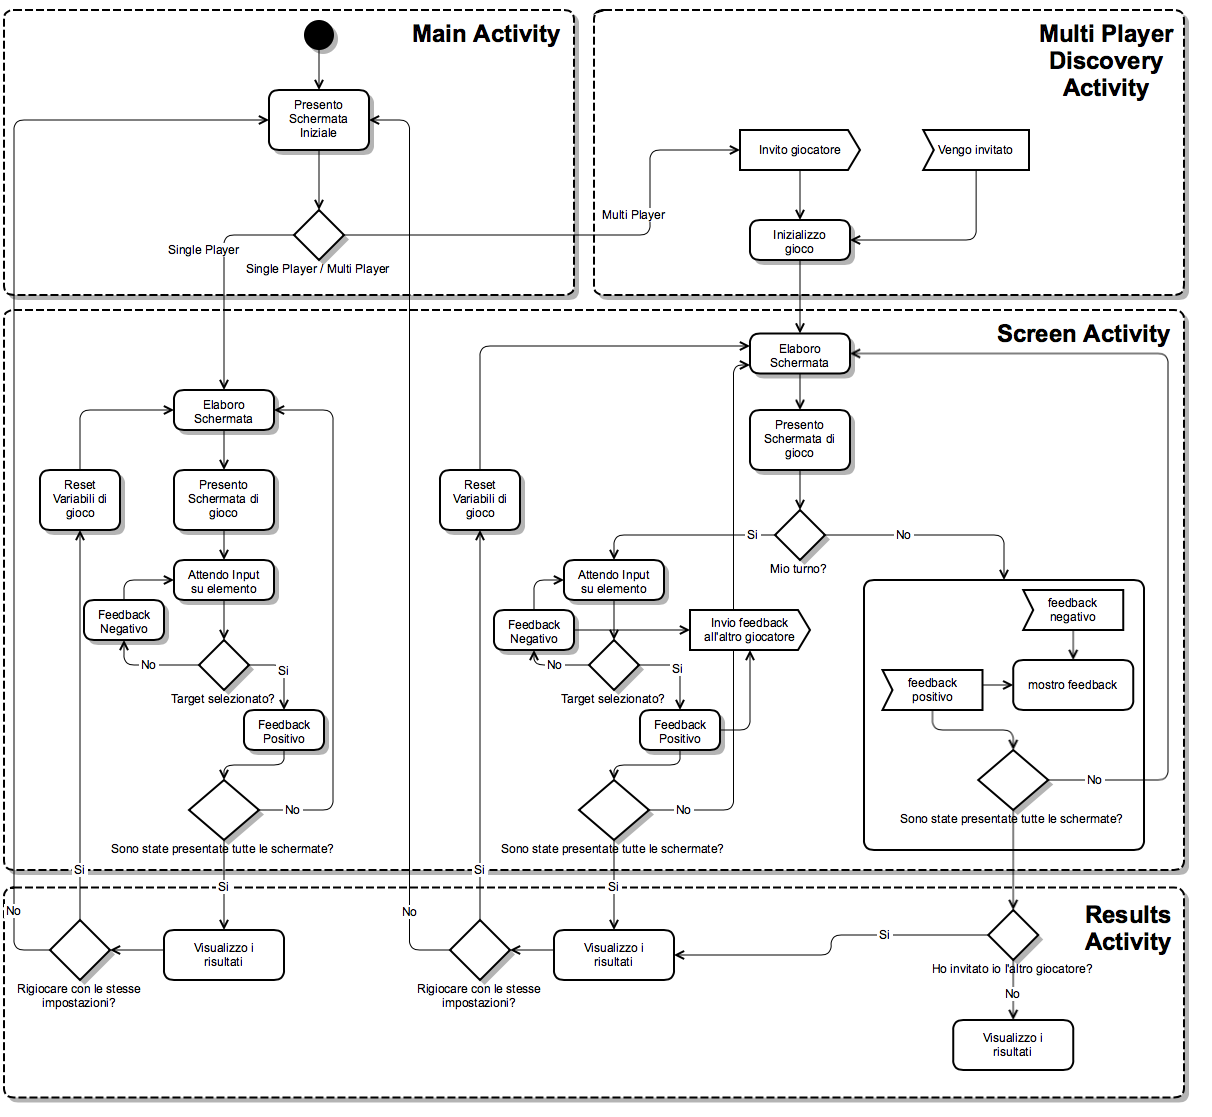
\includegraphics[width=13.5cm]{trova_l_intruso_android}
	\caption{Class Diagram}
	\label{fig:activity_diagram}
\end{figure}

%\subsection{Inizializzazione di una partita mutliplayer}

%\noindent Il sequence diagram
